\chapter{Results}

To obtain high quality electron diffraction the number of atoms available needs to be maximised and they need to be located in the smallest possible volume with a highly stable distribution. In order to achieve these goals with the \gls{odt} it is first necessary to establish a high density \gls{mot} cloud with a temperature of order one tenth the \gls{odt} depth. \Gls{mot} optimisation is beyond the scope of this project but nethertheless it is important to measure the \gls{mot} characteristics in order to be able to optimise the final characteristics of the \gls{odt}. Measurements of the \gls{odt} are necessary for the analysis and optimisation of the \gls{odt} parameters. The results of the \gls{mot} and \gls{odt} measurements are described here.

\section{Magneto-Optic Trap Analysis}
Analysis of the \gls{mot} allows us to optimise the \gls{mot} characteristics and the \gls{odt} parameters to achieve the best performance for the \gls{caes}. The temperature and number of trapped atoms in the \gls{mot} were calculated as shown below.

\subsection{Temperature}
Knowing the temperature of the \gls{mot} allows optimisation of the parameters of the \gls{odt} and can be useful for optimising the \gls{mot} itself. The procedure for calculating the temperature was discussed in section \ref{temp_measurement}. The data for this measurement was collected by releasing the \gls{mot}, waiting for a number of milliseconds and then imaging the cloud.

A program was created to perform this calculation\footnote{Written in Python, approximately 400 lines long.}. The data is first read from its binary storage format into the program. The data was rotated in order to align the long and short axes of the elliptically shaped \gls{mot} cloud with the $x$ and $y$ axes. A two dimensional, elliptical Gaussian distribution was then fitted to each of these images (see figure \ref{fig:mot_example_images} for examples). The 1/e radius of each of these distributions was used to fit to equation \ref{eq:cloud_radius} and the temperature was calculated with equation \ref{eq:temp_velocity}. The separate values for $x$ and $y$ were then averaged. The errors from the Gaussian fits combined with the error from the fit to equation \ref{eq:cloud_radius} were used to calculate the uncertainty. The results of this program are given below and the fitting is shown in figure \ref{fig:temp_fits}.

\begin{figure}[h]
\begin{subfigure}[b]{0.5\textwidth}
    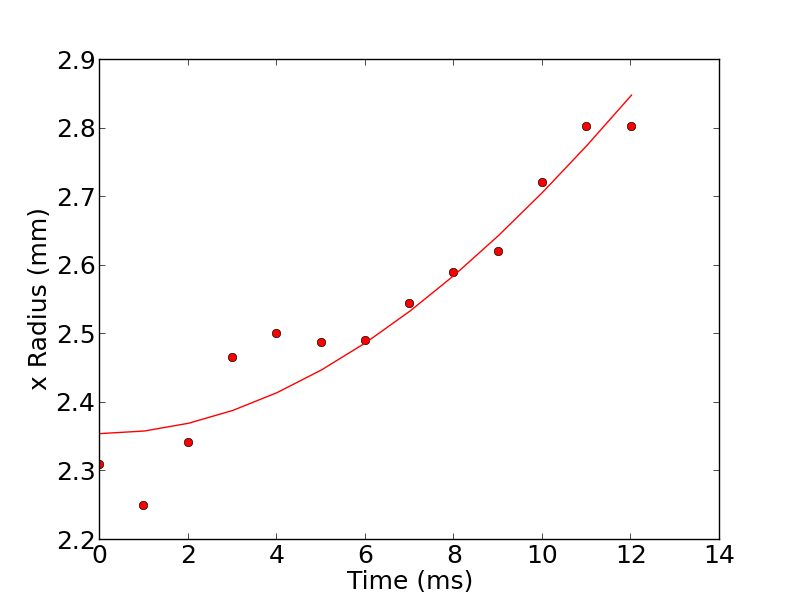
\includegraphics[width=\textwidth]{figs/final_temp_fitting_x.png}
\end{subfigure}\begin{subfigure}[b]{0.5\textwidth}
    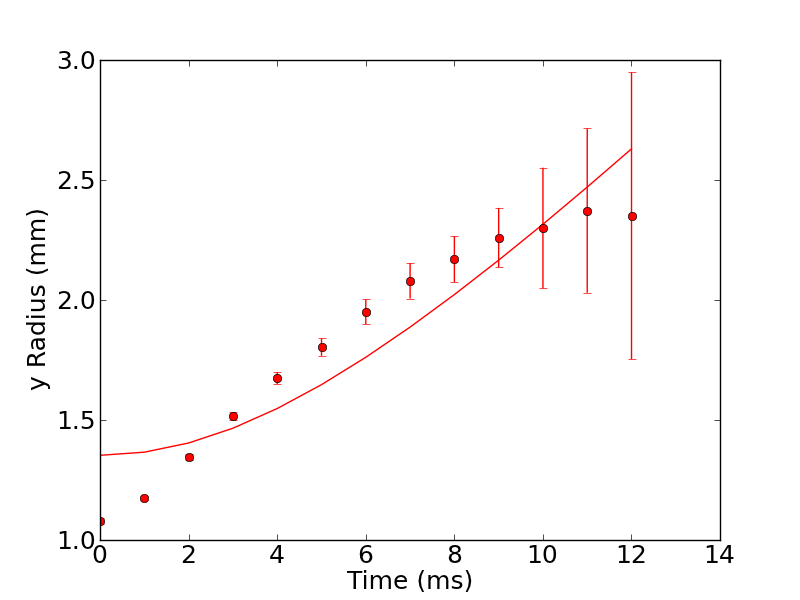
\includegraphics[width=\textwidth]{figs/final_temp_fitting_y.png}
\end{subfigure}
\caption{Measurements of thermal expansion of the MOT atom cloud (red points) and the fitted curve (red line).}
\label{fig:temp_fits}
\end{figure}

The temperature of the \gls{mot} was determined to be $139\pm22\,\unit{\mu K}$. Since the previous measurements of $70\,\unit{\mu K}$\cite{sheludko_shaped_2010} the detuning of the \gls{mot} cooling beams has been increased to optimise the loading rate and temperature scales with the detuning.

\subsection{Atom Count}
\label{mot_atom_count}
The number of atoms in the \gls{mot} is a critical metric as this determines the number of atoms available for loading into the \gls{odt} and thus for ionisation. The theory involved in determining the atom number is discussed in section \ref{atom_count}. The imaging laser intensity is well above saturation in the centre beam and thus equation \ref{eq:atom_count} must be used.

Another program was created to perform this calculation\footnote{Written in Python, approximately 200 lines long.} and data used for the temperature measurements was analysed. The number of atoms counted remains fairly constant until the cloud reaches the limits of the \gls{ccd} field of view after which there is a steep decline in the atom count (\ref{fig:mot_atom_count}). The number of atoms in the \gls{mot} is therefore $(1.3 \pm0.2)\times10^8$ which is comparable to measurements made previously with the \gls{caes}\cite{sheludko_shaped_2010}.

\begin{figure}[t]
\centering
    \begin{subfigure}[b]{0.3\textwidth}
    \centering
\begin{tikzpicture}
    \node[anchor=south west,inner sep=0] (image) at (0,0) {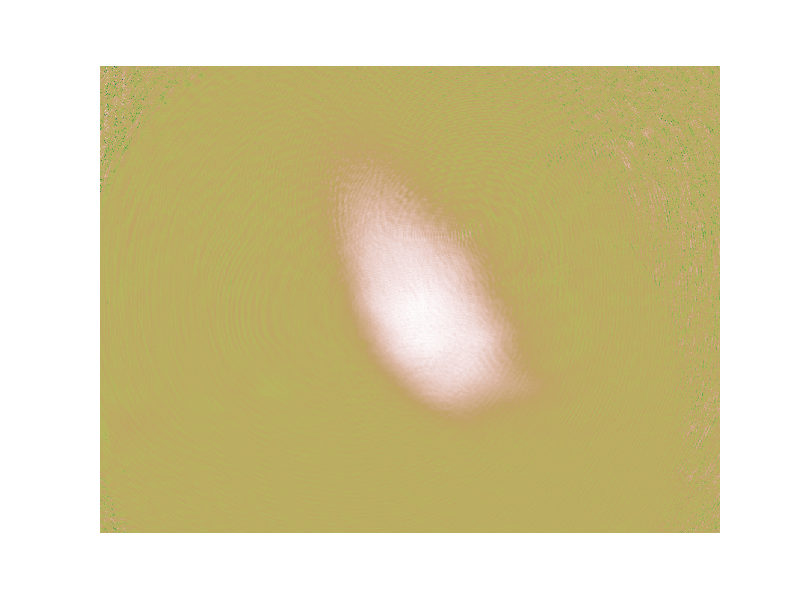
\includegraphics[width=0.8\textwidth]{figs/MOTimage1.png}};
    \begin{scope}[x={(image.south east)},y={(image.north west)}]
        \draw[black,thick] (0.2,0.15) -- node[above]{$5\,\unit{mm}$} (0.49524,0.15);
    \end{scope}
\end{tikzpicture}
\begin{tikzpicture}
\node[anchor=south west,inner sep=0] (image) at (0,0) {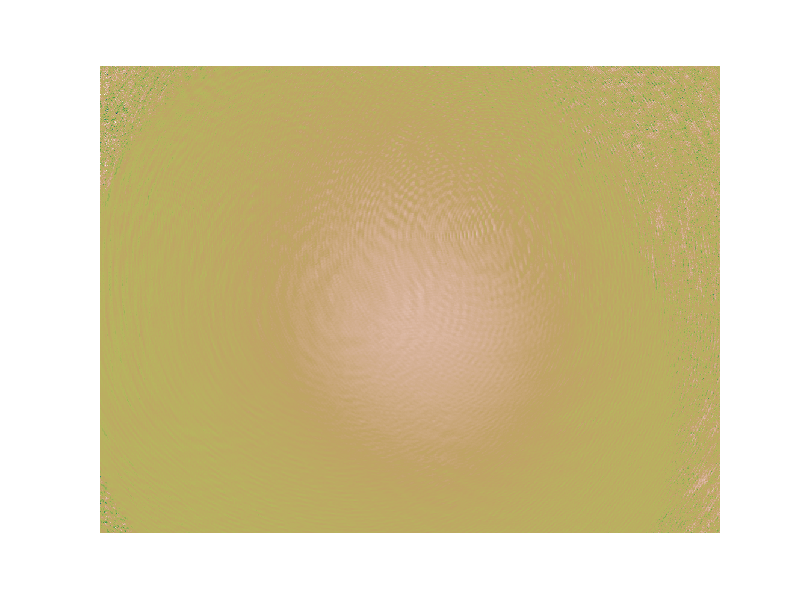
\includegraphics[width=0.8\textwidth]{figs/MOTimage2.png}};
    \begin{scope}[x={(image.south east)},y={(image.north west)}]
        \draw[black,thick] (0.2,0.15) -- node[above]{$5\,\unit{mm}$} (0.49524,0.15);
    \end{scope}
\end{tikzpicture}

    \caption{False colour absorption images of the MOT $1\,\unit{ms}$ (top) and $9\,\unit{ms}$ (bottom) after release.}
    \label{fig:mot_example_images}
    \end{subfigure}~~~\begin{subfigure}[b]{0.6\textwidth}
    \centering
    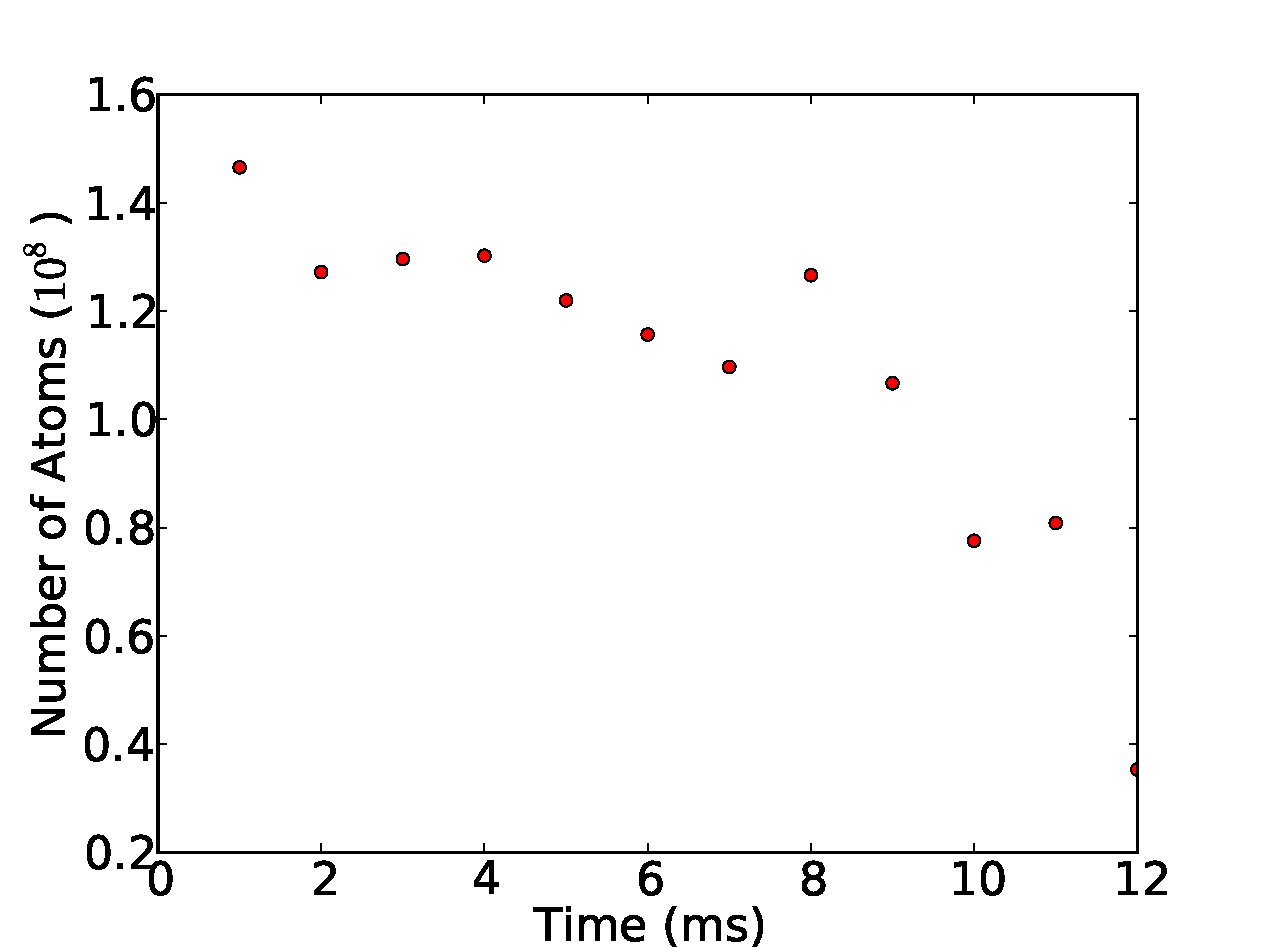
\includegraphics[width=0.8\textwidth]{figs/MOT_atom_count.pdf}
    \caption{The evolution of the number of atoms in the MOT cloud imaged by the camera during thermal expansion.}
    \label{fig:mot_atom_count}
    \end{subfigure}
    \caption{}
\end{figure}

\section{Optical Dipole Trap Analysis}
The first optical dipole trapping was observed in September 2012 and the first crossed \gls{odt} images acquired in early October 2012. Crossed trapping was observed as shown in figure \ref{fig:ODTimage1}.

An interesting effect can be observed in the crossed \gls{odt} images. Atoms within the \gls{odt} region can be seen extending along the beams driven by the scattering force of the trapping laser while leaving the core of the \gls{odt} behind. This is shown in figure \ref{fig:crossed_effect}. This effect implies that the \gls{odt} is not deep enough to trap all of the atoms within the trapping region and that the scattering rate is large as is expected with this detuning. This can be fixed by either increasing the depth of the \gls{odt} or reducing the temperature of the \gls{mot}.

The \gls{odt} absorption images were acquired by turning off the \gls{mot} trapping while the \gls{odt} was on. The atoms that were trapped in the \gls{mot} begin to expand thermally while those that are trapped in the \gls{odt} do not. An absorption image was acquired at certain times after the \gls{mot} trapping had ceased. This scenario was repeated with the \gls{odt} turned off for the entire process and this image was used as $I_0$ in equation \ref{eq:transmission_function_1}. This process is not perfect however as most of the atoms in the \gls{odt} are also present in the background image. AAs can be seen from the images however this technique is adequate for the initial calculations performed here.

The same set of data was used for all of the analysis performed in this section. In this data set the \gls{odt} laser was tuned to $\lambda=780.317\,\unit{nm}$ and it had only $358\,\unit{mW}$ of power. The \gls{mot} trapping was turned off for a range of times before imaging occurred.

\begin{figure}[h]
    \centering
    \begin{subfigure}[b]{0.3\textwidth}
\begin{tikzpicture}
    \node[anchor=south west,inner sep=0] (image) at (0,0) {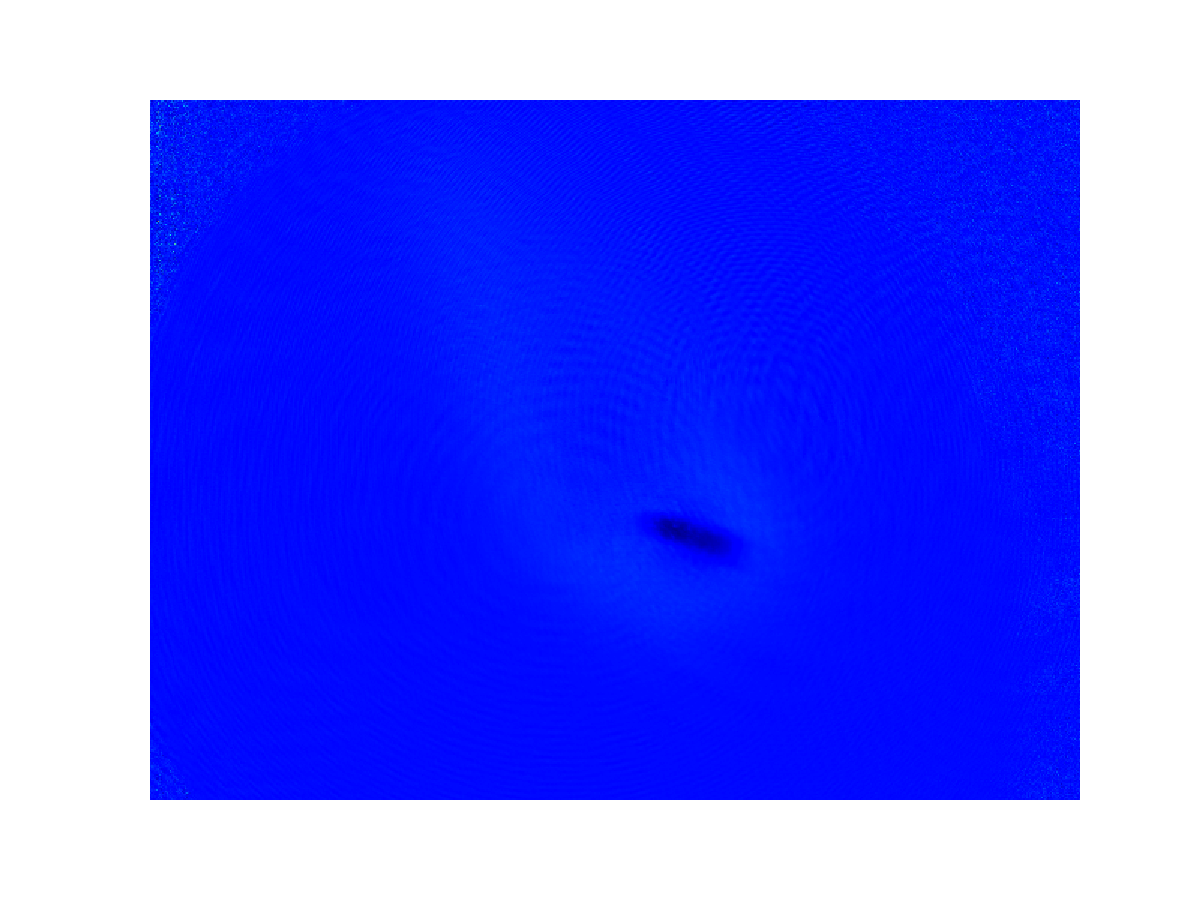
\includegraphics[width=1\textwidth]{figs/ODTimage1.pdf}};
    \begin{scope}[x={(image.south east)},y={(image.north west)}]
        \draw[white,thick] (0.2,0.15) -- node[above]{$5\,\unit{mm}$} (0.49524,0.15);
    \end{scope}
\end{tikzpicture}
    \end{subfigure}\begin{subfigure}[b]{0.3\textwidth}
\begin{tikzpicture}
    \node[anchor=south west,inner sep=0] (image) at (0,0) {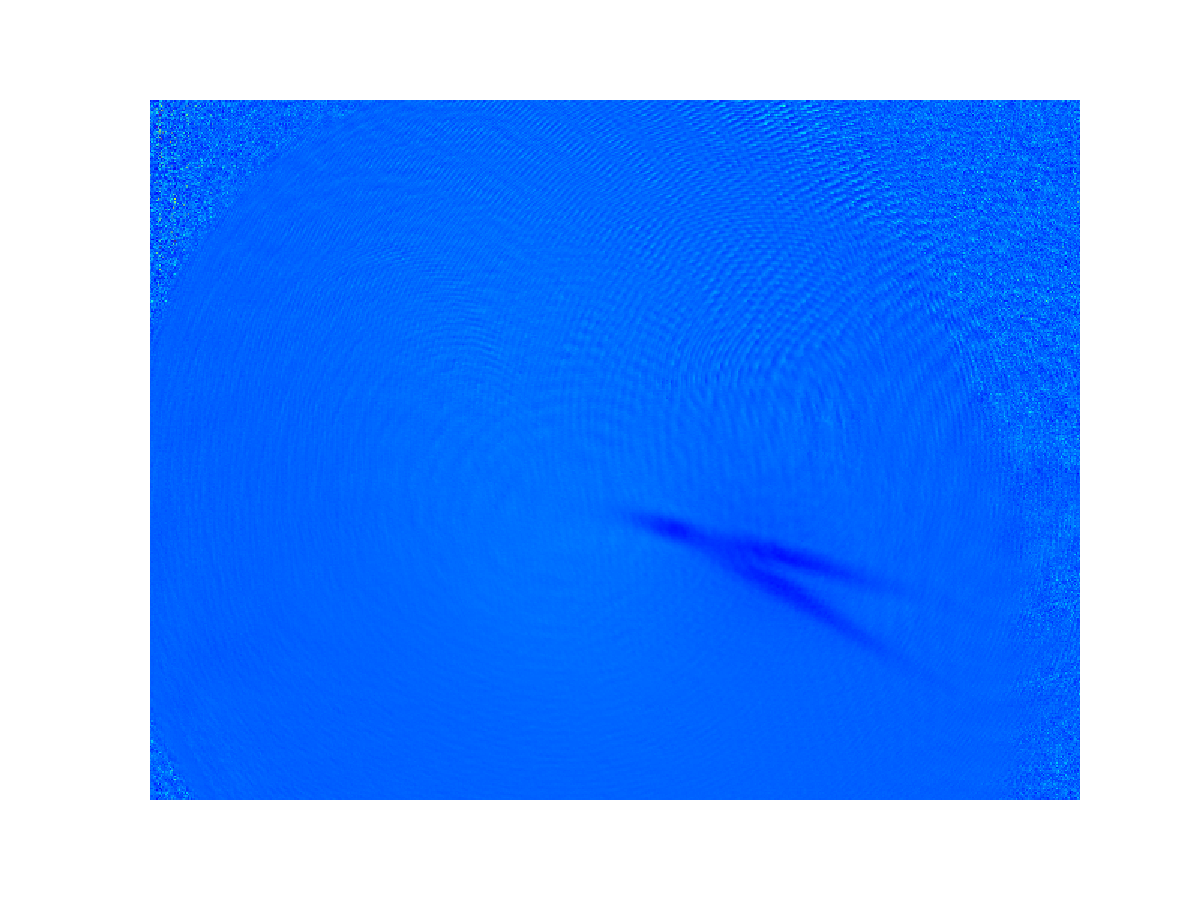
\includegraphics[width=1\textwidth]{figs/ODTimage2.pdf}};
    \begin{scope}[x={(image.south east)},y={(image.north west)}]
        \draw[white,thick] (0.2,0.15) -- node[above]{$5\,\unit{mm}$} (0.49524,0.15);
    \end{scope}
\end{tikzpicture}
    \end{subfigure}\begin{subfigure}[b]{0.3\textwidth}
\begin{tikzpicture}
    \node[anchor=south west,inner sep=0] (image) at (0,0) {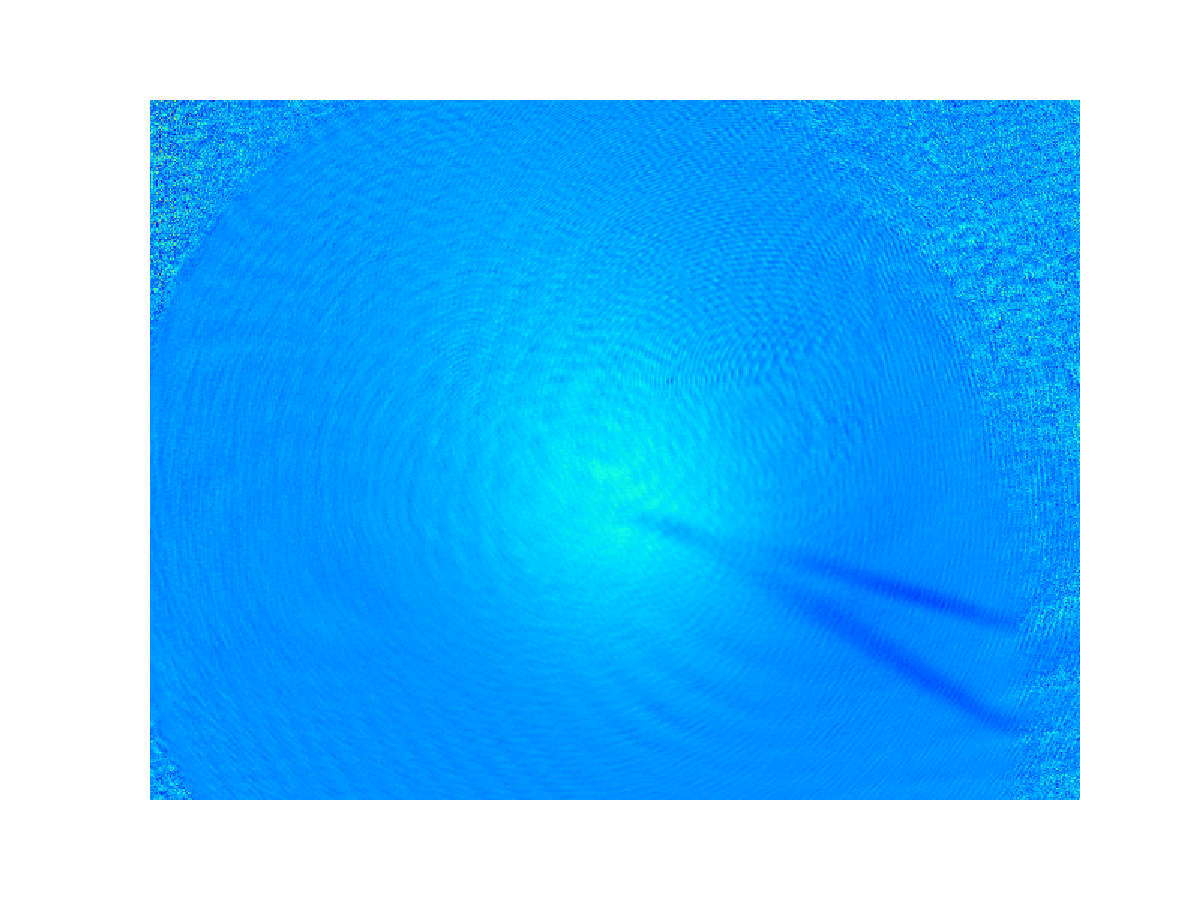
\includegraphics[width=1\textwidth]{figs/ODTimage3.pdf}};
    \begin{scope}[x={(image.south east)},y={(image.north west)}]
        \draw[white,thick] (0.2,0.15) -- node[above]{$5\,\unit{mm}$} (0.49524,0.15);
    \end{scope}
\end{tikzpicture}
    \end{subfigure}
\caption{False colour absorption images of a crossed ODT showing untrapped atoms in the region of the ODT being pushed down the trapping beams. The centre of the crossed ODT can be seen roughly in the centre of the first image. The untrapped atoms can be seen being pushed down the beam from the ODT region to the bottom right of the images.  The two beams of the ODT are visible due to the slightly off vertical imaging. The images are taken 2, 4 and $6\,\unit{ms}$ after the MOT trapping has be turned off.}
\label{fig:crossed_effect}
\end{figure}

\subsection{Size}
The size of the atom cloud in the crossed \gls{odt} can be calculated by fitting Gaussian curves to the distributions in the absorption images (figure \ref{fig:ODTimage1}). Taking the 1/e radius from the fit the length of the trap was found to be $1.3\pm0.15\,\unit{mm}$ and the width to be $0.4\pm0.02\,\unit{mm}$. The \gls{mot} trapping was turned off for $2\,\unit{ms}$ before imaging. Another program was created to do this analysis\footnote{Written in Python, approximately 300 lines long.}.

No data has been acquired that allows the atom distribution in the third axis (vertical) to be determined so the size in this axis is unknown. However due to the steep angle of the \gls{odt} beams it is reasonable to assume that the vertical trapping has a greater `length' than the trapping in the $x$ direction of figure \ref{fig:ODTimage1}.

\begin{figure}[h]
\centering
    % row 1
    \begin{subfigure}[b]{0.5\textwidth}\centering
\begin{tikzpicture}
    \node[anchor=south west,inner sep=0] (image) at (0,0) {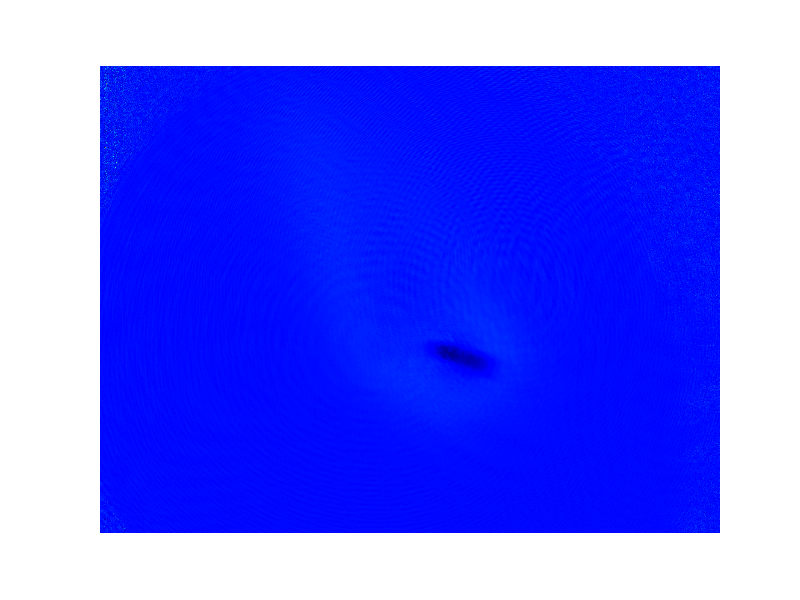
\includegraphics[width=0.7\textwidth]{figs/ODTimage1.png}};
    \begin{scope}[x={(image.south east)},y={(image.north west)}]
        \draw[white,thick] (0.2,0.15) -- node[above]{$5\,\unit{mm}$} (0.49524,0.15);
    \end{scope}
\end{tikzpicture}
        \caption{False colour absorption image of the crossed ODT.}
    \end{subfigure}~~~\begin{subfigure}[b]{0.5\textwidth}\centering
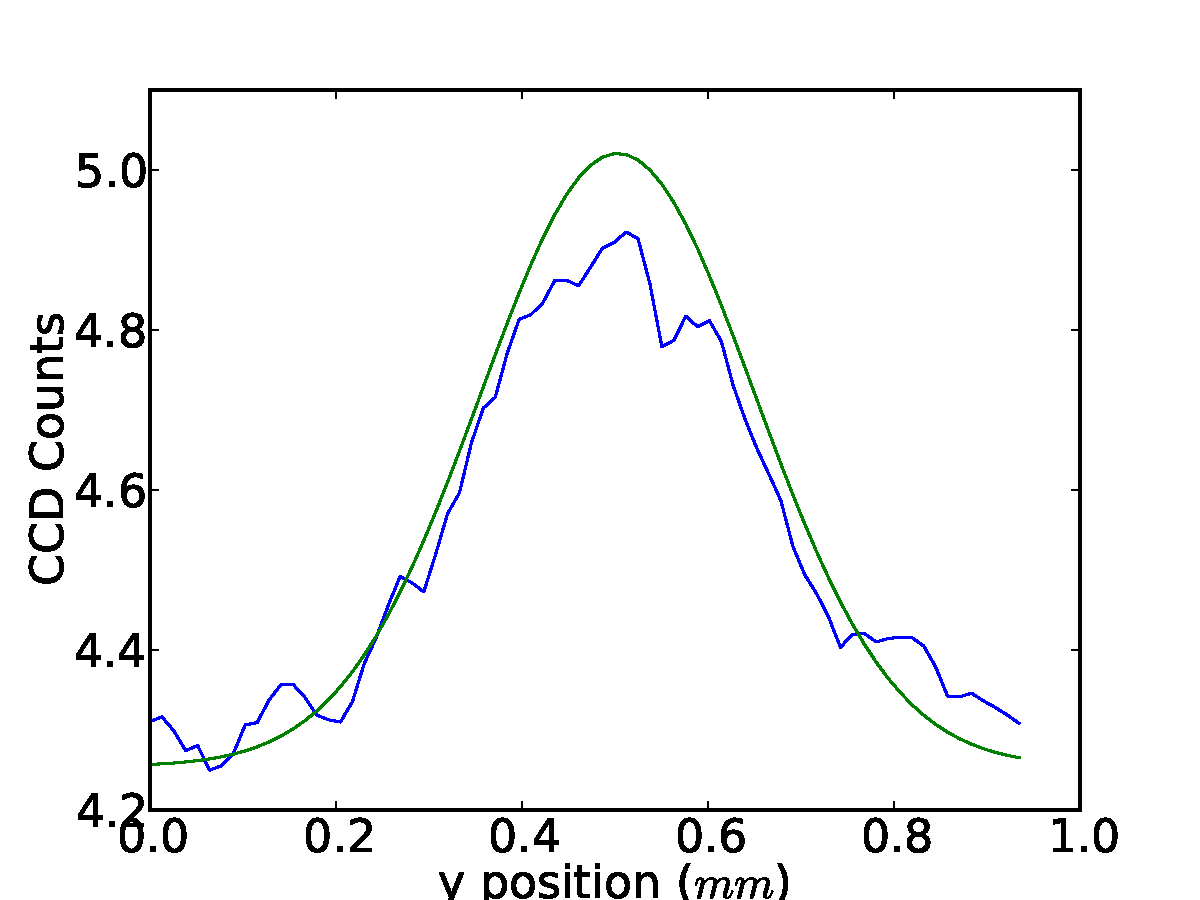
\includegraphics[width=0.7\textwidth]{figs/ODTimage1y.pdf}
        \caption{Vertical cross-section through the centre of the atom cloud in the ODT along with the fitted Gaussian.}
    \end{subfigure}


    % row 2
    \begin{subfigure}[b]{0.5\textwidth}\centering
        \begin{tikzpicture}
    \node[anchor=south west,inner sep=0] (image) at (0,0) {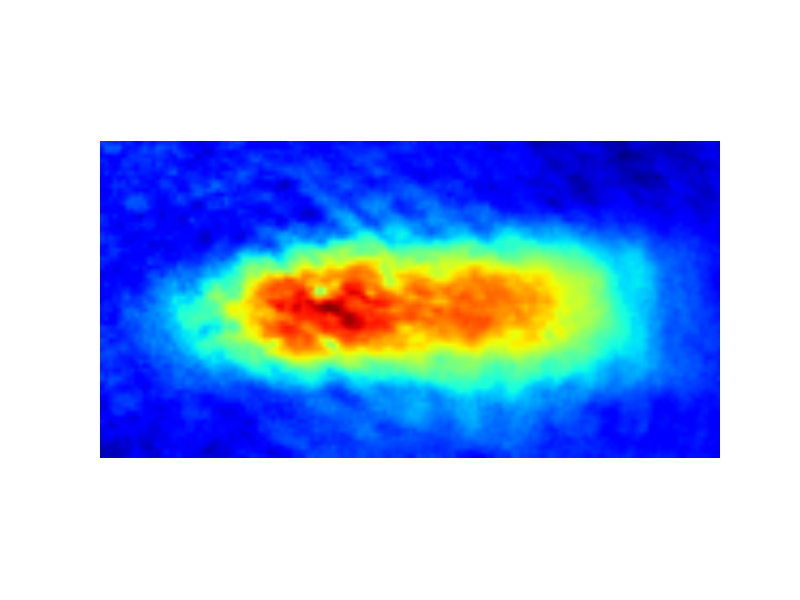
\includegraphics[width=0.9\textwidth]{figs/ODTimage1zoom.png}};
    \begin{scope}[x={(image.south east)},y={(image.north west)}]
        \draw[white,thick] (0.2,0.73) -- node[below left]{\footnotesize $1\,\unit{mm}$} (0.7351,0.73);
    \end{scope}
\end{tikzpicture}
\caption{A close up of the atom cloud shown in (a). The top left corner of this image is the origin for (c) and (d).}
    \end{subfigure}~~~\begin{subfigure}[b]{0.5\textwidth}
        \centering
        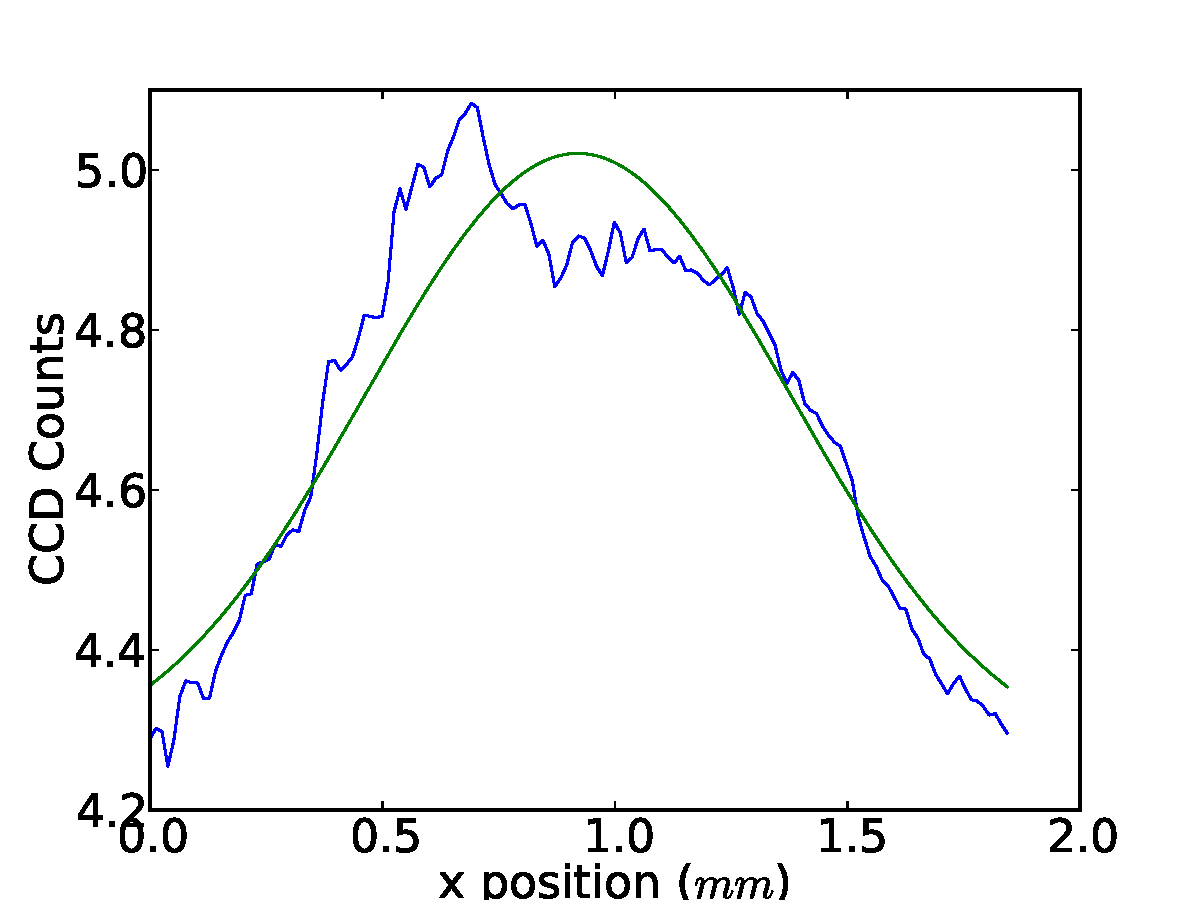
\includegraphics[width=0.7\textwidth]{figs/ODTimage1x.pdf}
        \caption{Horizontal cross-section through the centre of the atom cloud in the ODT along with the fitted Gaussian.}
    \end{subfigure}

    \caption{}
    \label{fig:ODTimage1}
\end{figure}


\subsection{Atom Count}
The number of atoms in the \gls{odt} can be calculated using the same methods and program used in section \ref{mot_atom_count} with slight modifications.

As mentioned above the \gls{mot} cloud is still expanding during the collection of this data so the number of residual atoms must be taken into account. This is done by using the atom-free image as a background ($I_0$) combined with an image of the expanding \gls{mot} ($I_{mot}$) and an image of the expanding \gls{mot} with the \gls{odt} turned on ($I_{mot+odt}$). Both images were acquired at the same time delay after the \gls{mot} was released. This provides us with the number of atoms in the expanding \gls{mot}, $N_{mot}$, and the number of atoms in the expanding \gls{mot} with the \gls{odt} turned on, $N_{mot+odt}$. Thus we can calculate the number of atoms in the \gls{odt}, $N_{odt}=N_{mot+odt}-N_{mot}$. Again this is not a perfect calculation as many of the atoms trapped in the \gls{odt} are taken from the \gls{mot} distribution however it is sufficient as preliminary data.

As shown in figure \ref{fig:lifetime} the number of atoms in the dipole trap at $t=0$ is $6.05\times10^6$ which corresponds to approximately 5\% of the atoms trapped in the \gls{mot}.

\subsubsection{Lifetime}
Measurement of the lifetime of the \gls{odt} is important since the \gls{caes} requires a high number of atoms available for ionisation several milliseconds after the \gls{mot} trapping has been turned off. Ideally the \gls{odt} will have a lifetime well in excess of $10\,\unit{ms}$. The simple model described in section \ref{lifetime_section} has been used to determine the 1/e lifetime of the \gls{odt} using another program\footnote{Written in Python, approximately 150 lines long.}. The lifetime has been calculated to be $2.1\pm0.9\,\unit{ms}$ with the wavelength and power detailed at the start of this section.

\begin{figure}[h]
\centering
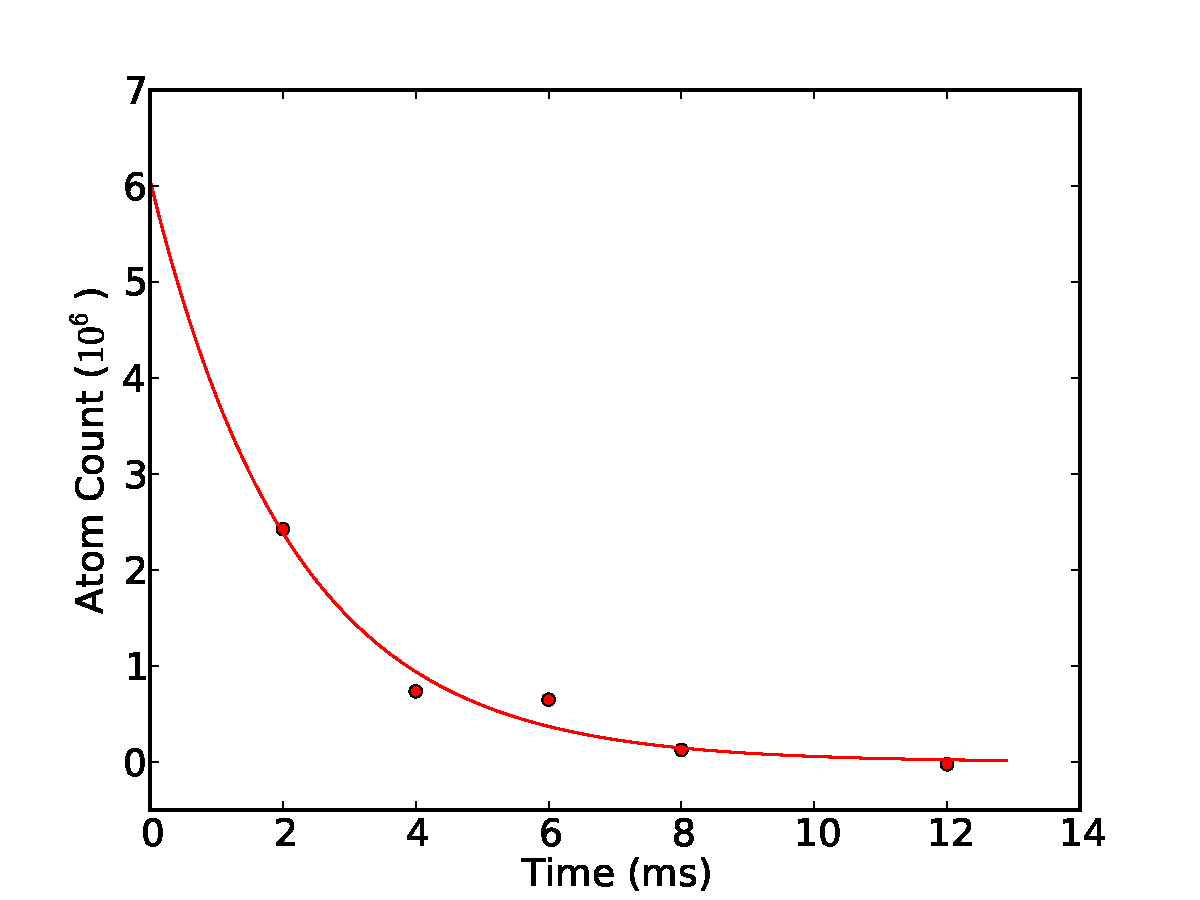
\includegraphics[width=0.6\textwidth]{figs/lifetime.pdf}
\caption{Number of atoms in the ODT over time. The initial number of atoms is $6.05\times10^6$ and the 1/e lifetime is $2.1\pm0.9\,\unit{ms}$.}
\label{fig:lifetime}
\end{figure}

\section{Summary}

Thes measurements establish a viable \gls{odt} with approximate dimensions of $1.3\,\unit{mm}$ by $0.4\,\unit{mm}$ initially holding $6.05\times10^6$ atoms with a lifetime of $2.1\,\unit{ms}$. These results are already sufficient to demonstrate the use of the \gls{odt} for electron diffraction experiments, currently in progress.
